%\documentclass[12pt,letterpaper,final]{article}
\documentclass[12pt,letterpaper,final]{article}
\usepackage[latin1]{inputenc}
\usepackage{amsmath}
\usepackage{amsfonts}
\usepackage{amssymb}
\usepackage{graphicx}
\usepackage{fullpage}
\usepackage{cite}
\author{H.S. Barnard}
\title{Preliminary Design Report: Electron beam EDX analysis for magnetic fusion devices}
\begin{document}
\maketitle
%\abstract{Abstract Abstract Abstract Abstract Abstract }

\section{Introduction}

Plasma material interactions (PMI) is a critical area of study for magnetic fusion devices.  Understanding the effects of PMI including erosion, deposition, fuel retention, and impurity production all play a vital role in the development of fusion reactors. The successful demonstration of the accelerator-based in-situ materials surveillance (AIMS) diagnostic clearly shows that particle beam based in-situ diagnostics can provide measurements of the effects of PMI with unprecedented spatial and temporal resolution.

AIMS is essentially a novel in-situ implementation of ion beam analysis (IBA) techniques that are used for materials analysis. The IBA used in AIMS is similar to particle induced gamma emission (PIGE) and nuclear reaction analysis (NRA) for low-Z elements. The current application of AIMS is effective for measuring low-Z elements.

To expand on this concept, a similar technique using electron beams can be used for in-situ analysis to provide a complementary set of high-Z measurements. This technique similar to energy dispersive X-ray spectroscopy (EDX or EDS) which is commonly used in electron microscopy. The overlap between the techniques will allow the development of electron AIMS to draw from decades of EDS experience and refinement.

\section{Energy dispersive X-ray (EDX) analysis}

Background on EDS analysis...

\section{In-situ tokamak EDX}

The goal of tokamak EDX is to provide macroscopic EDX measurements with $\sim1$~cm spot size over the entire poloidal range of the tokamak wall and over significant fraction of the toroidal range. This is done using an electron beam (section \ref{sec:ElectronGun}) which scanned over the wall of the tokamak using the tokamak's magnetic field coils (section \ref{sec:BeamSteering} to induce X-rays in the material surface (section \ref{sec:BeamInteractions}. Spectroscopic analysis of these X-rays is performed, with energy dispersive detectors (section \ref{sec:detectors}) to provide quantitative analysis of the elemental composition of the surface. 

When EDX is used in microscopy there is relatively small variation in detection geometry throughout the spatial range of measurements due to the small beam deflections (nm-$\mu$m scale). For tokamak EDX however, the macroscopic (cm-m scale) dimensions of the measurements make modeling of the beam and detector geometry challenging. With the experience and simulation tools developed for the AIMS diagnostic, tokamak EDX can be achieved using modern electron beam and X-ray detection technology.

\subsection{Beam steering and modeling}
\label{sec:BeamSteering}
Like AIMS, the tokamak's magnetic fields are used to the electron beam to target PFCs for analysis. Compared to a $\sim 1$~MeV ion beam, the magnetic field required to steer an electron beam with energy in the relevant range for EDX (10-100~keV) along an identical trajectory is substantially less. This can be seen by comparing the magnetic rigidity $R$ for a beam used for AIMS to an electron beam (shown in figure \ref{fig:Rigidity}. Magnetic rigidity is defined as $B\rho = R(T)$, providing the relationship between the radius of curvature $\rho$, the applied magnetic field $B$, and the beam's kinetic energy $T$.

\begin{figure}[!h]
 \centering
  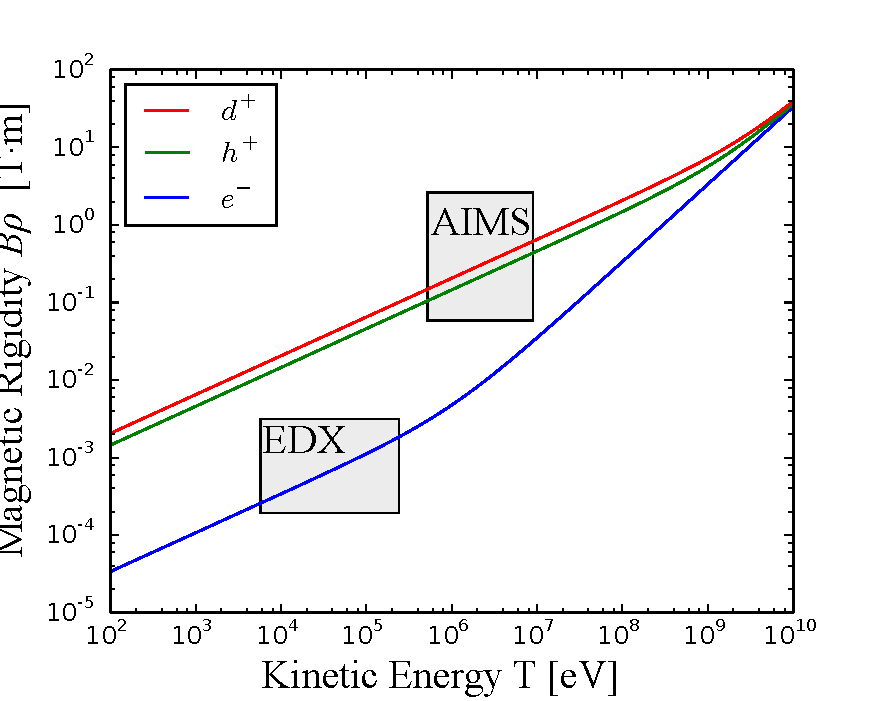
\includegraphics[width=\columnwidth]{figures/MagneticRigidity.pdf}
 \caption{Magnetic rigidity is shown versus kinetic energy for ion beams and electron beams. Magnetic rigidity $R$ relates radius of curvature $\rho$ and the applied magnetic field $B$ such that $B\rho = R(E)$. The shaded areas indicate the operating energy range for EDX and AIMS.}
 \label{fig:Rigidity}
\end{figure}

\textbf{... More on beam simulation...}

\section{Beam interactions with materials}
\label{sec:BeamInteractions}
Electron beams interacting with matter are more complicated than ion beams. Ion beams are relatively simple to model because the ions lose energy approximately monotonically with distance with minimal straggling. Electron beams, however, interact primarily through large-angle scattering and undergo many scattering, atomic excitation, and ionization events before either coming to rest or exiting the material surface. As a result, Monte Carlo methods are often used to study electron beams to predict the energy and spatial distribution of the electron trajectories as well as the X-ray emission. 

Analysis was performed for this study using CASINO 2.48 \cite{CASINO}, a Monte Carlo (MC) simulation package developed for electron microscopy and EDX. The complexity of the of the electron scattering can be seen from figure~\ref{fig:ElectronsInTarget}.

\begin{figure}[!h]
 \centering
  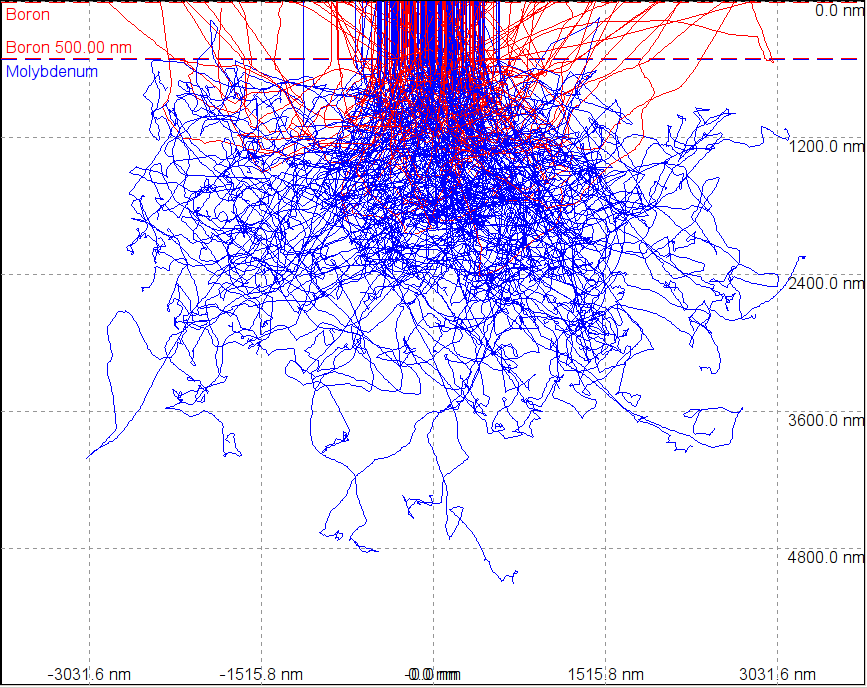
\includegraphics[width=\columnwidth]{figures/ElectronsInTargetWide.png}
 \caption{Monte Carlo simulation of electrons interacting with a boron coated molybdenum target, generated with CASINO 2.48 \cite{CASINO}. A 1~$\mu$m diameter beam is shown to keep the beam size comparable to the scattering length scales within the target. Red trajectories represent electrons that backscatter and exit the material surface. Blue trajectories represent electrons that come to rest within the material.}
\label{fig:ElectronsInTarget}
\end{figure}

\subsection{X-Ray excitation with electron beams}

For materials analysis, X-rays from K and L shell transitions are commonly used. These X-rays result from the transitions following inner shell ($n=1$) and second shell ($n=2$) ionization respectively. These X-rays are typically $\sim 1 - 100$~keV and are produced at distinct characteristic energies that are unique to each element.

The process of X-ray production from electron bombardment involves several effects that complicate the analysis. The K and L ionization cross sections are strongly dependant on electron energy. X-ray emission resulting from these ionization also competes with other de-excitation processes, particularly Auger electron emission. In addition, the X-rays are attenuated within the material. These effects can complicate the analysis but are readily accounted for in accounted for in the MC simulation. The main consequence is for the measurement is that Auger electrons must be obstructed or deflected so they do not interfere with the detector.

\subsection{Backscattered Electrons}

As electrons from the beam penetrate the material and substantial fraction of them backscatter out of the material surface after one or more collisions.  For electrons scattering off of molybdenum the backscattering coefficient is $N_e/N_{e,\mathrm{backscattered}} \approx	0.3$ for normal incidence and tends to increase with incident angle. Backscattering is important to consider because many of the electrons that leave the surface have sufficient energy to produce X-rays elsewhere in the within the vessel. This is seen in the backscattered electron energy spectrum shown in figure~\ref{fig:BackscatteringSpectrum}.

\begin{figure}[!h]
 \centering
  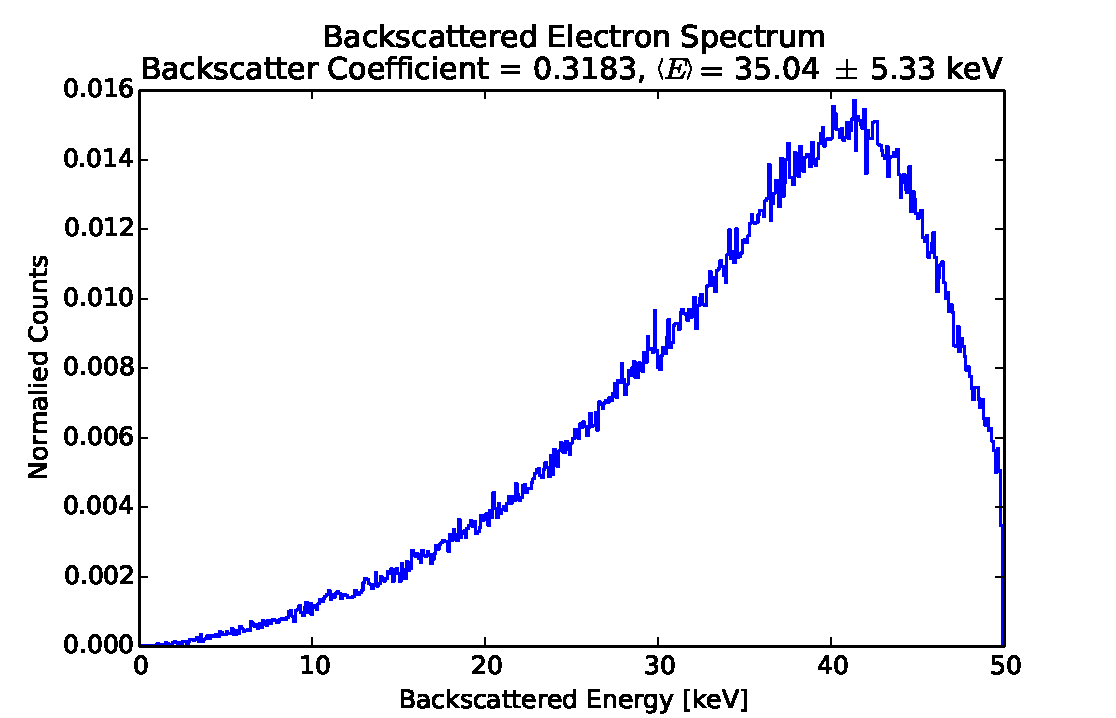
\includegraphics[width=\columnwidth]{figures/MolybdenumBackscatteringSpectrum.pdf}
 \caption{Electron backscattering spectrum for 50~keV electrons with normal incidence on molybdenum.} 
 \label{fig:BackscatteringSpectrum}
\end{figure}

For 50~keV electron on molybdenum, nearly 1/3 of the electrons are backscattered with a mean energy of 35~keV. This is sufficient to produce X-rays when these electrons interact with other surfaces. In order to make spatially resolved EDX measurements, it is therefore necessary to shield the detector from X-rays resulting from backscattering. Methods of shielding these X-rays and electrons from the detector are described in section~\ref{sec:DetectionGeometry}.

\section{Tokamak EDX Hardware}
Performing EDX in a tokamak has some engineering challenges but is possible with presently available technology. This sections overviews the required hardware that will be necessary to perform tokamak EDX with discussion of the engineering that is involved.

\subsection{Electron beam accelerator}
\label{sec:ElectronGun}
Electron beams have been studied and used for nearly a century for many applications in science and industry. As a result, there are many electron accelerators or electron guns, that are available spanning the necessary parameter range for EDX. For example electron accelerators from electron microscopes are regular used for EDX high degree of precision, but produce relatively low X-ray intensities because of their limited beam current. Unlike EDX commonly used in microscopy, analysis in a tokamak does not require a highly focused $\sim$nm beam spot. Therefore, beam current limitations due beam power density can be relaxed from $\sim$nA used in microscopy to higher currents in the $\mu$A to mA range. As a result, if higher X-ray production rates are desired, there are a variety of DC and pulsed electron guns that have been developed in industry for heat treatment, welding, machining, and melting/evaporation processes. These accelerators can have beam energies up to 300~keV with beam currents in up to the $>$1~mA range \cite{HammHamm}.

An example of an electron accelerator that could be readily used for tokamak EDX is the EGH-6002 electron gun from Kimball Physics \cite{KimballPhysics} shown in figure \ref{fig:ElectronGun}. This device has independently adjustable beam energy (1~keV to 50~keV), beam current (10~nA to 100$\mu$A), and spot size (0.5 mm to 100 mm). A higher current option is also available allowing for 10~nA to 10~mA. The spot size is controlled with internal optics designed for a working distance of 50~mm to 1000~mm. With these optics $<$1~cm spatial resolution should be achievable in tokamaks like Alcator C-Mod.

\begin{figure}[!h]
 \centering
  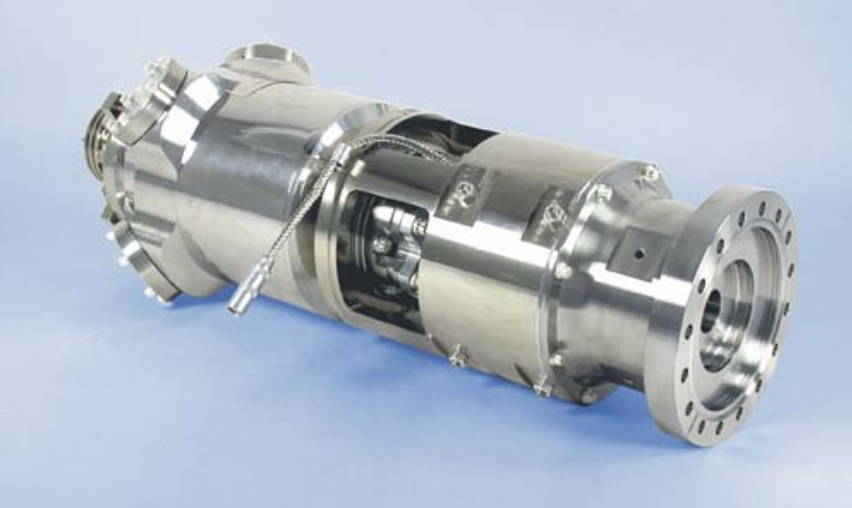
\includegraphics[width=\columnwidth]{figures/ElectronGunEGH6002.png}
 \caption{Photo of a commercially available electron gun from Kimball Physics~\cite{KimballPhysics}. The model EGH-6002 electron gun has the following specifications. Beam energy: 1~keV to 50~keV (adjustable), Beam current: 10~nA to 100 $\mu$A (adjustable), spot-size: 0.5~mm to 100~mm (adjustable with built-in optics), design working distance: 50~mm to 1000~mm.}
 \label{fig:ElectronGun}
\end{figure}

\subsection{Detectors}
\label{sec:detectors}
Lithium drifted silicon detectors (SiLi) also, often referred to as silicon drift detectors (SDD), are commonly used for X-ray spectroscopy in the range of 1~keV to tens of keV. Modern detectors are also available in compact sizes with thermoelectric refrigeration units to maintain their low operating temperatures $< 100$~K. Such detectors are commercially available. Examples from Amptek \cite{Amptek} are shown in figure \ref{fig:AmptekDetectors}.

\begin{figure}[!h]
 \centering
  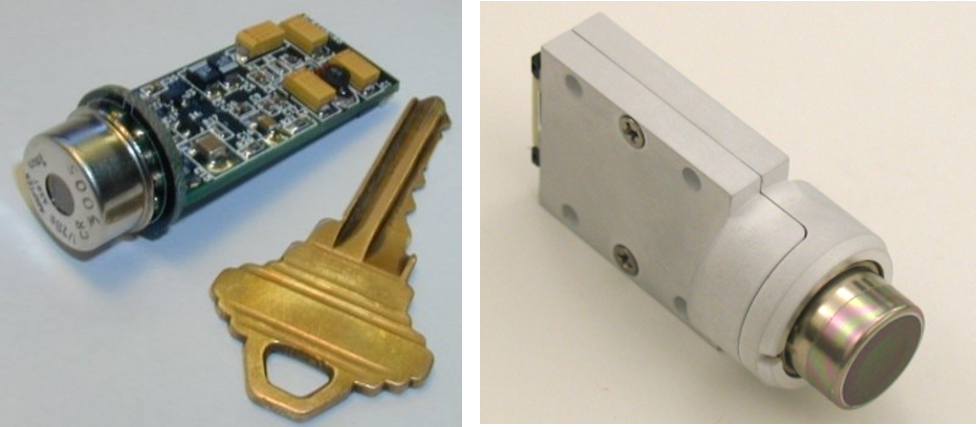
\includegraphics[width=\columnwidth]{figures/SDDPhoto_DoubleCol.pdf}
 \caption{Photos of silicon drift detectors from Amptek with attached pre-amplifier and packaging. Images reproduced from Amptek website \cite{Amptek}.}
 \label{fig:AmptekDetectors}
\end{figure}

X-ray detectors require the detection element to be hermetically sealed. As a result, the thickness of the and composition of the X-ray window covering the active 

\begin{figure}[!h]
 \centering
  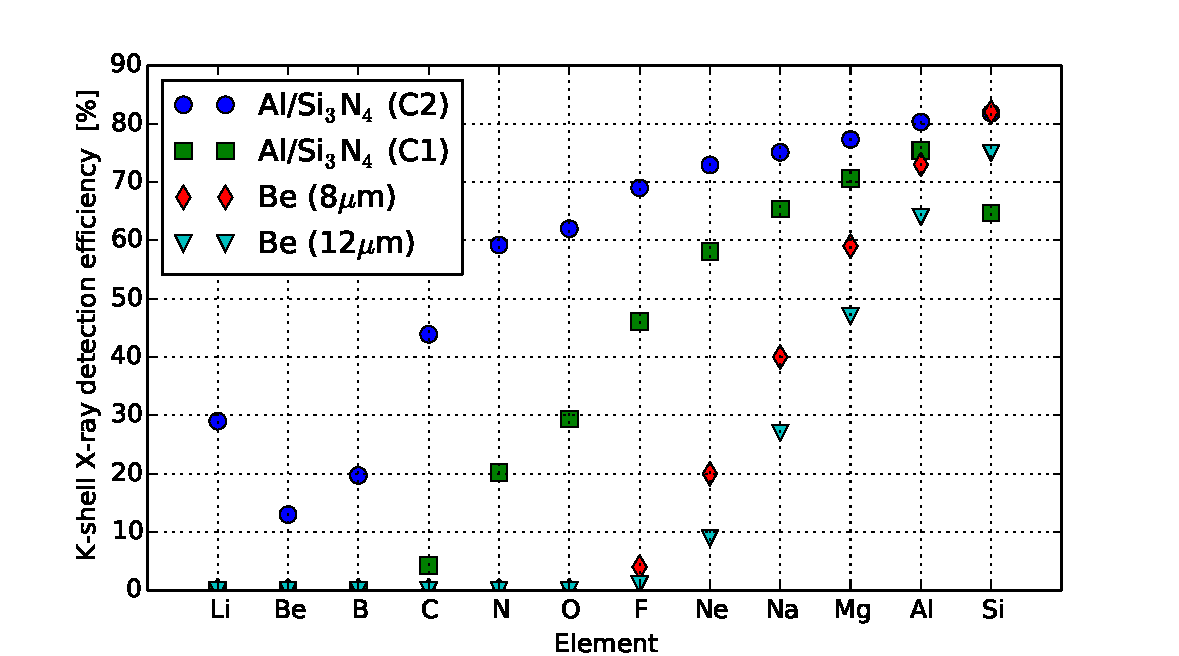
\includegraphics[width=\columnwidth]{figures/KShellDetectorEfficiency.pdf}
 \caption{X-ray windows covering detectors limits low energy X-Ray detection in silicon drift detectors. Detection efficiency for K-shell X-rays are shown for low-Z elements. Beryllium (Be) windows are compared to new window `C-series' windows from Amptek \cite{Amptek}. }
 \label{fig:DetectorEff}
\end{figure}

\subsection{Detection geometry}
\label{sec:DetectionGeometry}

Since the X-rays of interest typically have mean free paths of less than 100~$\mu$m, a line-of-sight path is required between the beam target and detector.  This can be achieved by two methods: 1) an array of fixed detectors that are located outside of the plasma region that are distributed poloidally to provide full coverage of target locations or 2) a retractable detector on a robotic arm that maintains close proximity to the beam target. The choice between both of these options is based on the beam current and the corresponding X-ray intensity. In both cases, detector positioning system is required to maintain proper detection angle to the beam target.
 
The detector must be protected from backscattered electrons and Auger electrons as well as the X-rays that they produce when interacting with surfaces far from the target. To remove the extraneous X-rays the detectors must have a collimator (e.g. a lead tube) that tracks the position of the beam target location. This can be accomplished with a remotely operated positioning device with 2 degrees of freedom. To prevent backscattered and Auger electrons from reaching the detector, the collimator in combination with electron deflecting permanent magnets can be used. This detector will require some engineering effort but is certainly achievable with technology from modern industrial robotics.

\section{Applications in Alcator C-Mod}

\subsection{Measurement of boron}

\begin{figure}[!h]
 \centering
  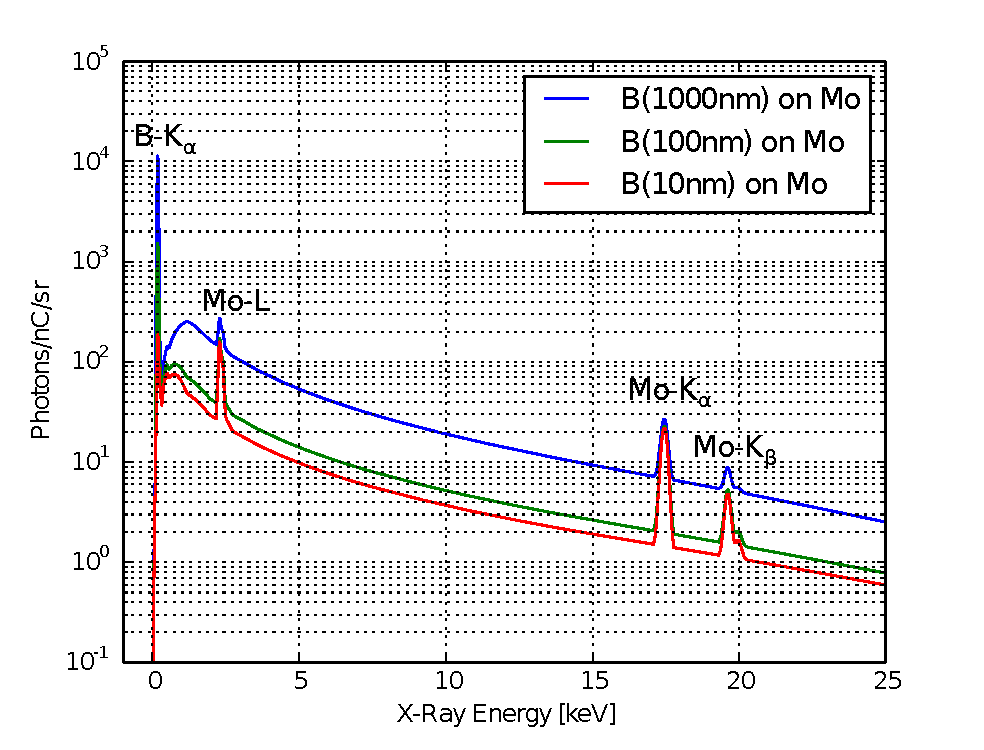
\includegraphics[width=\columnwidth]{figures/BoronOnMoSpectra.pdf}
 \caption{}
 \label{fig:BoronSpectra}
\end{figure}

\begin{figure}[!h]
 \centering
  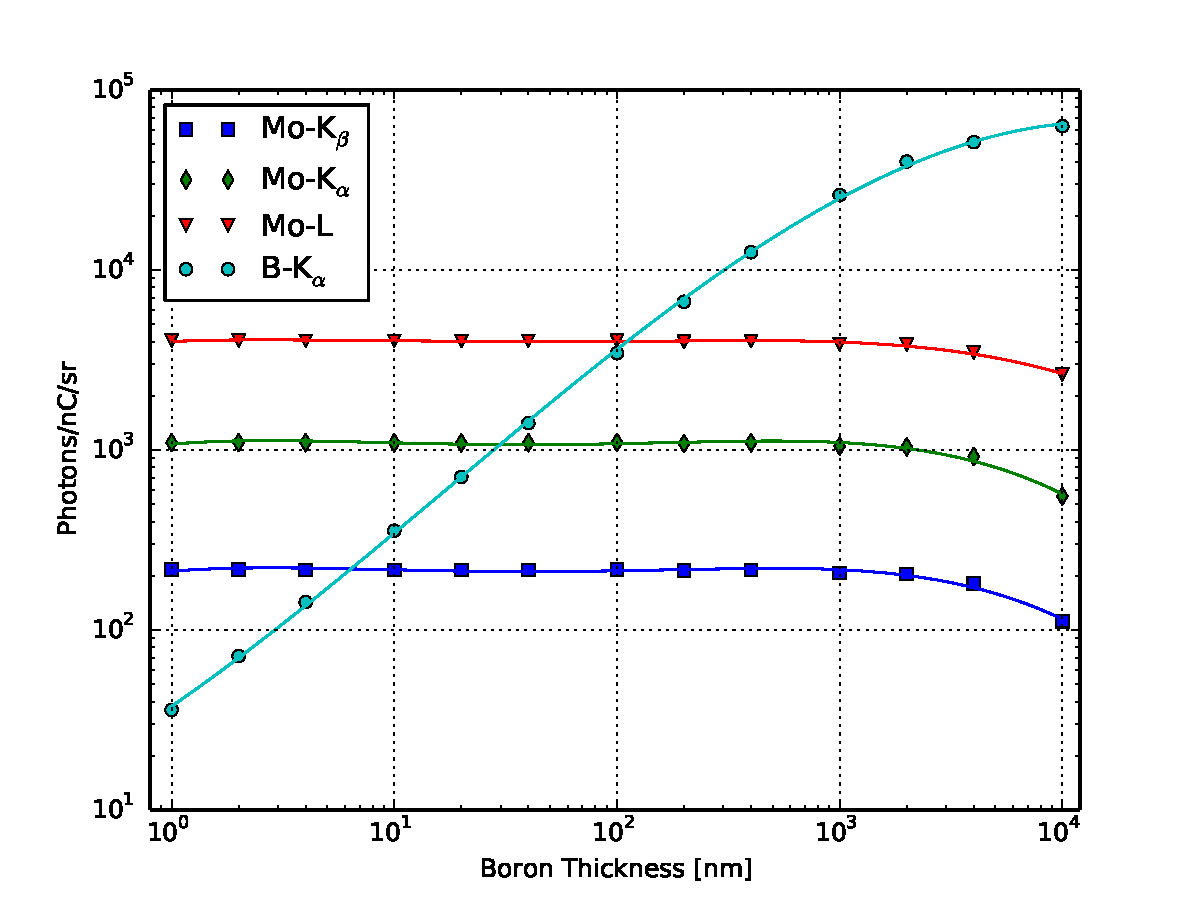
\includegraphics[width=\columnwidth]{figures/BoronLayerXRayIntensityVsThickness.pdf}
 \caption{}
 \label{fig:BoronIntensity}
\end{figure}

\subsection{In-direct measurement of surface layers}

\subsection{Depth-marker analysis}

Implanted depth markers can be used to measure net changes in surface thickness. A layer of dissimilar material can be inserted at well defined depth below a material surface through ion implantation or by a series of deposition processes. This layer or 'depth marker' will emit characteristic X-rays that are distinguishable from the bulk or the surface material. When the thickness of the surface above the depth marker changes, the intensity of the X-rays from the marker will change as a function of thickness due the effect of surface thickness on X-ray attenuation and average beam energy loss before reaching the depth of the marker. 

The X-ray intensity from the marker and its sensitivity to changes in thickness depend strongly on the X-ray energy, X-ray attenuation in the target material, and the relative X-ray intensity from the bulk of the target material. For maximum sensitivity, the marker material and depth should be optimized to make use of these effects.

\subsubsection{Depth Marker Design and Optimization}

The marker should be deep enough that a moderate amount of X-ray attenuation and beam energy loss occurs so that both effects contribute to the sensitivity of the measurement to surface changes. This is addressed by placing the marker at depth that is less than but comparable to the mean free path of the X-rays it produces. The marker must also produce enough X-rays to compete with emission from the bulk material, otherwise it will be difficult to resolve the marker's X-rays in a spectrum dominated by the bulk material. This can be addressed by using marker with as large an areal density as possible and by using an element that has a higher X-ray emission cross section than the bulk of the material.






\bibliographystyle{plain}
\bibliography{ElectronBeamAIMS.bib}
 
\end{document}
